\documentclass{article}
\usepackage[spanish]{babel}
\usepackage[numbers,sort&compress]{natbib}
\usepackage{graphicx}
\graphicspath{ {images/} }
\usepackage{subfigure}
\usepackage{url}
\usepackage{hyperref}
\usepackage{amsmath}
\usepackage[top=15mm, bottom=40mm, left=15mm, right=15mm]{geometry}
\setlength{\parskip}{2mm}
\setlength{\parindent}{0pt}
\usepackage{listings}
\usepackage{mathrsfs}


\lstdefinestyle{mystyle}{
  numbers= left}
\lstset{style=mystyle}

\author{3175}
\title{Práctica 12: Red Neuronal}
\date{\today}

\begin{document}

\maketitle


\section{Introducción}
Las Redes Neuronales son un campo muy importante dentro de la Inteligencia Artificial. Inspirándose en el comportamiento conocido del cerebro humano, trata de crear modelos artificiales que solucionen problemas difíciles de resolver mediante técnicas algorítmicas convencionales.
Las primeros ejemplos de redes neuronales artificiales aparecen al final de la década de los cincuenta y la referencia histórica más corriente es la que alude al trabajo realizado por $Frank Rosenblatt$ en un dispositivo denominado perceptrón \citep{web1}.
 
\section{Objetivo}
Mediante una red neuronal que es una demostración básica de aprendizaje de máquina se desea analizar el desempeño de la misma, tomando como objetivo reconocer dígitos de imágenes pequeñas en blanco y negro.
 
\section{Metodología}
Usando de base el código proporcionado \citep{webelisa}, Se usan perceptrones para determinar si el productp de $X$ y $w$(peso) es positiva en cuyo caso se determina como VERDADERO o si no FALSO. Para convertir un entero en una secuencia de bits que indican
cuáles potencias están presentes y cuáles están ausentes de la suma en donde los posibles residuos en división entre dos son solamente cero y uno), simplemente se prueban cuáles potencias le caben. 
Posteriormente se de usan 15 pixeles por dígito en un cuadro de $3*5$. Los cuales son determinados de manera probabilística para los 10 dígitos usando colores negro, gris, blanco modelados por un archivo CSV. 
\lstinputlisting[language= R, firstline=35, lastline=35]{P12.R}

Las probabilides para el color del pixeles negros de $0.995$ y $0.8$, los blancos $0.001$ y $0.1$, finalmente para los grises de $0.75$ y $0.65$.
Finalmente con referencia en el código\citep{web2}, se paralelizó la etapa de la prueba llamando a las funciones a los núcleos por medio del paquete $parSapply$ y se realizaron 30 réplicas:

\lstinputlisting[language= R, firstline=65, lastline=80]{P12.R}

\section{Resultados}
Los resultados de la efectividad de la red neuronal se midieron en base al porcentaje de contadores entre el número de pruebas para los distintos casos de probabilidad de los pixeles, para así notar que tan precisa es la red neuronal en base al modelo proporcionado (los dígitos).

\begin{figure}[!ht]
\centering
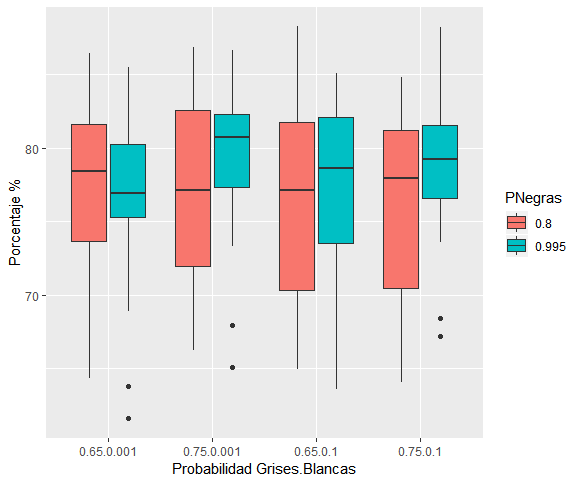
\includegraphics[width=17cm, height=8cm]{P12gt.png}
\caption{Porcentaje de precisión de la red neuronal con distintas probabilidades}
\end{figure}


\section{Conclusiones}
Se puede concluir que la mayoria de aciertos se presentó para las probabilidades de $0.995$ hablando de los píxeles negros, $0.75$ al referirnos a los píxeles grises y $0.001$ en el caso de los píxeles blancos. Probablemente debido a que la mayoria de los píxeles de los modelos eran negros o grises y en menor medida blancos, por eso se encontraron favorecidas las probabilidades altas en los blancos y grises, y la menor en los blancos. Se pueden hacer pruebas posteriores con distintas iteraciones y modelos para corroborar éstas afirmaciones.

\bibliographystyle{plainnat}
\bibliography{biblio12}
\end{document}